\chapter[New Loss Functions]{New Loss Functions: Comparing Asymmetric and Symmetric Methods of Evaluating Error} \label{ch3:loss}
\chaptermark{New Loss Functions}
\setlength{\epigraphwidth}{4.5in}
\epigraph{Maybe all one can do is hope to end up with the right regrets.}{Arthur Miller, \textit{``The Ride Down Mount Morgan''}, 1991}

%----------------------------------------------------------------------------------------------------------------------------------------------------------------------------------------------------------
\section*{Summary}
In practice, the loss function for a chosen statistical learning method is the translation of a informal philosophical objective into the formal language of mathematics \cite{hennig2007some}. Therefore, the choice of a loss function in estimation is somewhat subjective and depends on the specific application of the model or the decisions being made when using it. Some loss functions have already been established in and are common in hydrology. 

This chapter will look at differences in performance of already established and new functions in hydrology when they are embedded in the machine learning algorithm rather than using them as only an evaluation step after the model is built. 

%----------------------------------------------------------------------------------------------------------------------------------------------------------------------------------------------------------
\section{Introduction}
% add literature review here
Mechanistic models in hydrology simulate conditions based on available input parameters, modeled processes, and calibration to specific locations. \textit{Measures-of-fit} or the similarity of the simulations to the observations help in assessing model performance. Visual similarity is recommended first (i.e., the plot of observed and simulated time series), and calculated measures-of-fit are recommended next. In model calibration, these measures can help guide better fits of simulations to observations.  

In statistical learning, the same process can be used by estimating the model using a pre-defined loss function, solve the simulation problem as well as is possible, and then calculate the model measures-of-fit of interest. However, improving a model trained on a different loss function than that which is desired can be quite tricky. Since the machine learning algorithm requires a loss function to begin with, we can directly define the custom loss function as the measure-of-fit of interest before deploying the learning algorithm. This section performs statistical learning with different loss functions, and then examines the differences in predictions. 

Typical loss functions in statistical learning are the $\ell1-norm$ and $\ell2-norm$ (See Equation \ref{eq:l1} and \ref{eq:l2}). The $\ell2-norm$ is the familiar objective function in simple least-squares regression, a convex function, emphasizing points distant from the bulk of the data. % (i.e., data points that have high leverage and can influence the model more than other points).

\begin{equation} \label{eq:l1}
	\ell_1(y_i,\hat{f}(x_i)) = ||y_i-\hat{f}(x_i)||_1 = \abs{y_i-\hat{f}(x_i)} 
\end{equation}
	
\begin{equation} \label{eq:l2}
	\ell_2(y_i,\hat{f}(x_i)) = ||y_i-\hat{f}(x_i)||_2^2 = \left(y_i-\hat{f}(x_i)\right)^2 
\end{equation}
 
% IS THIS TRUEEEEEEE? 
% If we use equation \ref{eq:l1}, the algorithm will try to correctly predict the median correctly, and if we use equation \ref{eq:l2}, the algorithm will try to correctly predict the mean. Both imply that the modeler is more concerned with the measures of centrality than predicting the extremes of the distribution more accurately.

\textit{Risk}, or cost, is defined as the expectation of the loss function. For example, the risk of over predicting the severity of a drought can be defined as \textit{how much} it was over predicted on average. This distance can be defined as the absolute value of the difference or the difference squared as in Equations \ref{eq:l1risk} and \ref{eq:l2risk}, the empirical risks associated with the  $\ell1-norm$ and $\ell2-norm$. The expectation of the $\ell2-norm$ will produce a model that regresses to the mean, and the $\ell1-norm$ regresses to the median. That is, the $\ell2-norm$ is more sensitive to outliers than the $\ell1-norm$.

\begin{equation} \label{eq:l1risk}
	\begin{aligned}
		& L_1(y_i,\hat{f}(x_i)) = E\left[\ell_1(y_i, \hat{f}(x_i))\right] = \frac{1}{n} \sum_{i=1}^{n} \abs{y_i-\hat{f}(x_i)}
		% E\left[\abs{y_i-\hat{f}(x_i)}\right] \\
		% & L\left(\abs{y-\hat{f}(x)}\right) = \frac{1}{n} \sum_{i=1}^{n} \abs{y_i-\hat{f}(x_i)}
	\end{aligned}
\end{equation}
	
\begin{equation} \label{eq:l2risk}
	\begin{aligned}
		& L_2(y_i,\hat{f}(x_i)) = E\left[\ell_2(y_i, \hat{f}(x_i))\right] = \frac{1}{n} \sum_{i=1}^{n} {(y_i-\hat{f}(x_i))^2}
		% E\left[(y_i-\hat{f}(x_i))^2\right] \\
		% & L\left((y-\hat{f}(x))^2\right) = \frac{1}{n} \sum_{i=1}^{n} {(y_i-\hat{f}(x_i))^2}
	\end{aligned}
\end{equation}

On the other hand, \textit{Regret} is the difference between the consequences of a sub optimal decision and the optimal decision. Often, in reinforcement learning, the objective is to minimize regret, which is equivalent to maximizing the highest accumulated reward \cite{sutton2018reinforcement}. For example, maybe over predicting the severity of a drought this year will lead to better management of resources and fewer regrets in later years.

In this research, to avoid developing a mathematical representation for regret, we leave this discussion and proceed with the much simpler \textit{risk-minimization framework} (See Equation \ref{eq:mlriskmin}). 

\begin{equation} \label{eq:mlriskmin}
	\hat{f}(x_i) = \underset{\tilde{f}}{\mathrm{argmin}} \ E\left[L(y, \tilde{f}(x))\right] \\
\end{equation}
%----------------------------------------------------------------------------------------------------------------------------------------------------------------------------------------------------------
\section{Research Design} \label{ch4:design}
This study used the monthly unimpaired flows data set developed and maintained by the California Data Exchange Center (CDEC). Unimpaired flow is the flow produced by the basin in its current state, but, without dams and diversions \cite{cadwruf2016}. 

The data spans 69 California basins (See appendix \ref{d:ufdataset}, Figure \ref{fig:map}) from 1982 to 2014. It can be downloaded with the {\tt sharpshootR} package in R \cite{beaudette2016package}. 28 predictor attributes were calculated for each observation point based on the knowledge of basin characteristics and processes that influence a watershed's response to precipitation: evaporation (temperature); snowfall (cumulative sum of precipitation below 2$^{\circ}$C); storage in soil (with soil and land cover parameters); antecedent conditions (with lagged precipitation and temperature parameters); and groundwater processes (with geology and depth to a restricted layer) (See Table \ref{table:ufvariables}). The dataframe has approximately 18,500 monthly unimpaired flow observations in acre-feet (AF) and as a continuous variable can be used for regression type studies. 
% subset of the data, we just need to investigate the loss function. 
% Could be interesting to use the temperature dataset for this chapter too.
%Since we are just examining the loss function, the developed dataset is much smaller

Typical measures-of-fit developed in hydrologic modeling are the Mean Absolute Error (MAE), Relative Standard Deviation (RSD), Relative Mean (RMU), Mean Squared Error (MSE), Root Mean Square Error (RMSE), normalized RMSE (nRMSE), RMSE standard deviation ratio (RSR), Percent Bias (PBIAS), Coefficient of Determination (R$^2$), Nash-Sutcliffe Efficiency (NSE), Index of Agreement (d), Modified NSE, Modified d, Relative NSE, Relative d, King-Gupta Efficiency (KGE), and Volumetric Efficiency (VE). appendix \ref{e:mof} presents their equations, strengths, and weaknesses. First, let us consider a list of characteristics that the loss function, in its application to hydrologic prediction, should fulfill:

(1) \textbf{Should the loss function be symmetric?} In symmetric functions, under predicting produces the same loss as over predicting of the same absolute error. However, a conservative loss function applies a different penalty to the different directions of loss. That is, an asymmetric loss function can force the model to over predict the severity of floods and droughts rather than under predict them. This approach requires the labelling of all instances of the data as either a peak, normal, or drought point, requiring a labeling mechanism (i.e., a classification model) before running the predictive regression model. 

Great care should be taken not to introduce ``data leakage'', or the leakage of information from the response variable into the final predictive model; the classification model will have to either be trained on the predictor variables only, or use a portion of the data that is thrown away for the rest of the study. A simple classification model can be defined by a fit of a thin plate spline to the precipitation data with a predefined degree of smoothness (i.e., degree of freedom). Next, we find the points at which the direction of curvature (the second derivative) in the time series changes. Areas where the curvature is upward can be labelled drought and downward labelled flood. 

After all data points are labeled, we define two asymmetric loss functions for each peak and valley section (See Figure \ref{fig:asymmetric1}). Such loss functions can be defined as linear exponential (LINEX) loss if smoothness is desired (See Equation \ref{eq:linex}). However, current subgradient-based and derivative-free methods of optimization in convex programming can easily handle non-differentiability at the origin of the loss function. In fact, many asymmetric loss functions in machine learning have a simple \textit{kink} in them, which makes them otherwise entirely differentiable. Figure \ref{fig:asymmetric3} and Equation \ref{eq:asshinge} explain such a function. % For a definition of terms see appendix \ref{a:terms}. 

\begin{figure}[ht]
	\centering
	\begin{subfigure}{.5\textwidth}
  		\centering
 		 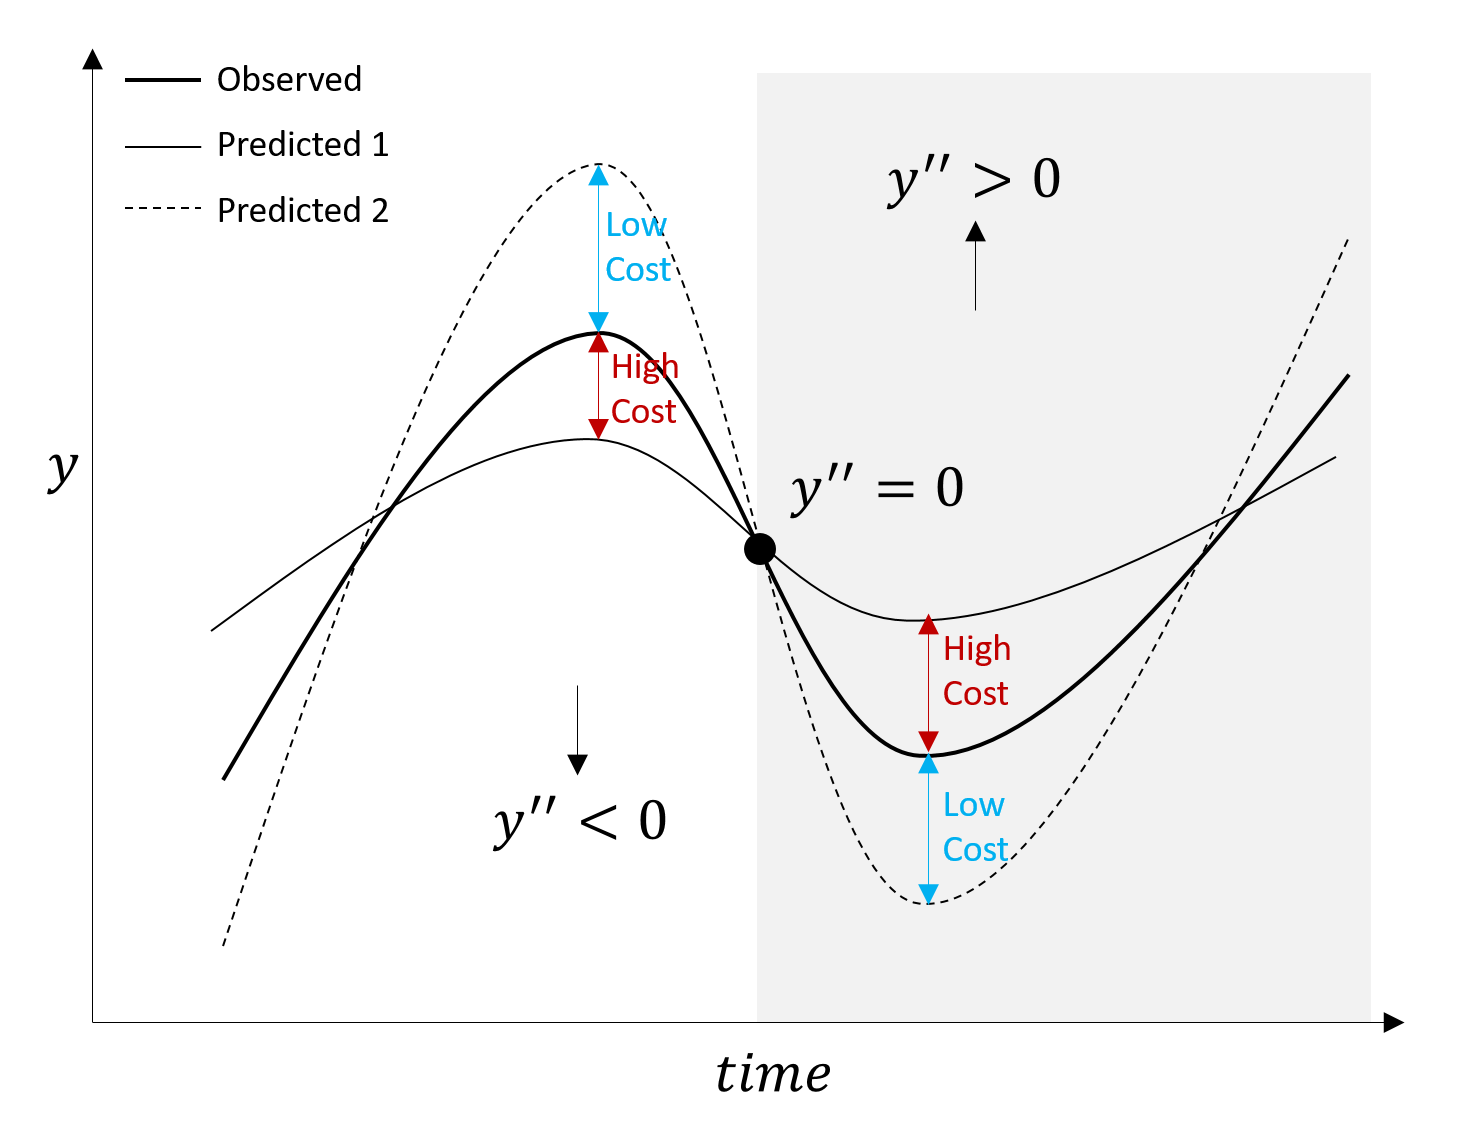
\includegraphics[width=\textwidth, trim={0 0 0 0}, clip=true]{plots/asymmetric1_a.png}
  		\caption{Asymmetric loss shown around peaks and valleys.\newline}
  		\label{fig:asymmetric1a}
	\end{subfigure}% 
	\begin{subfigure}{.5\textwidth}
  		\centering
  		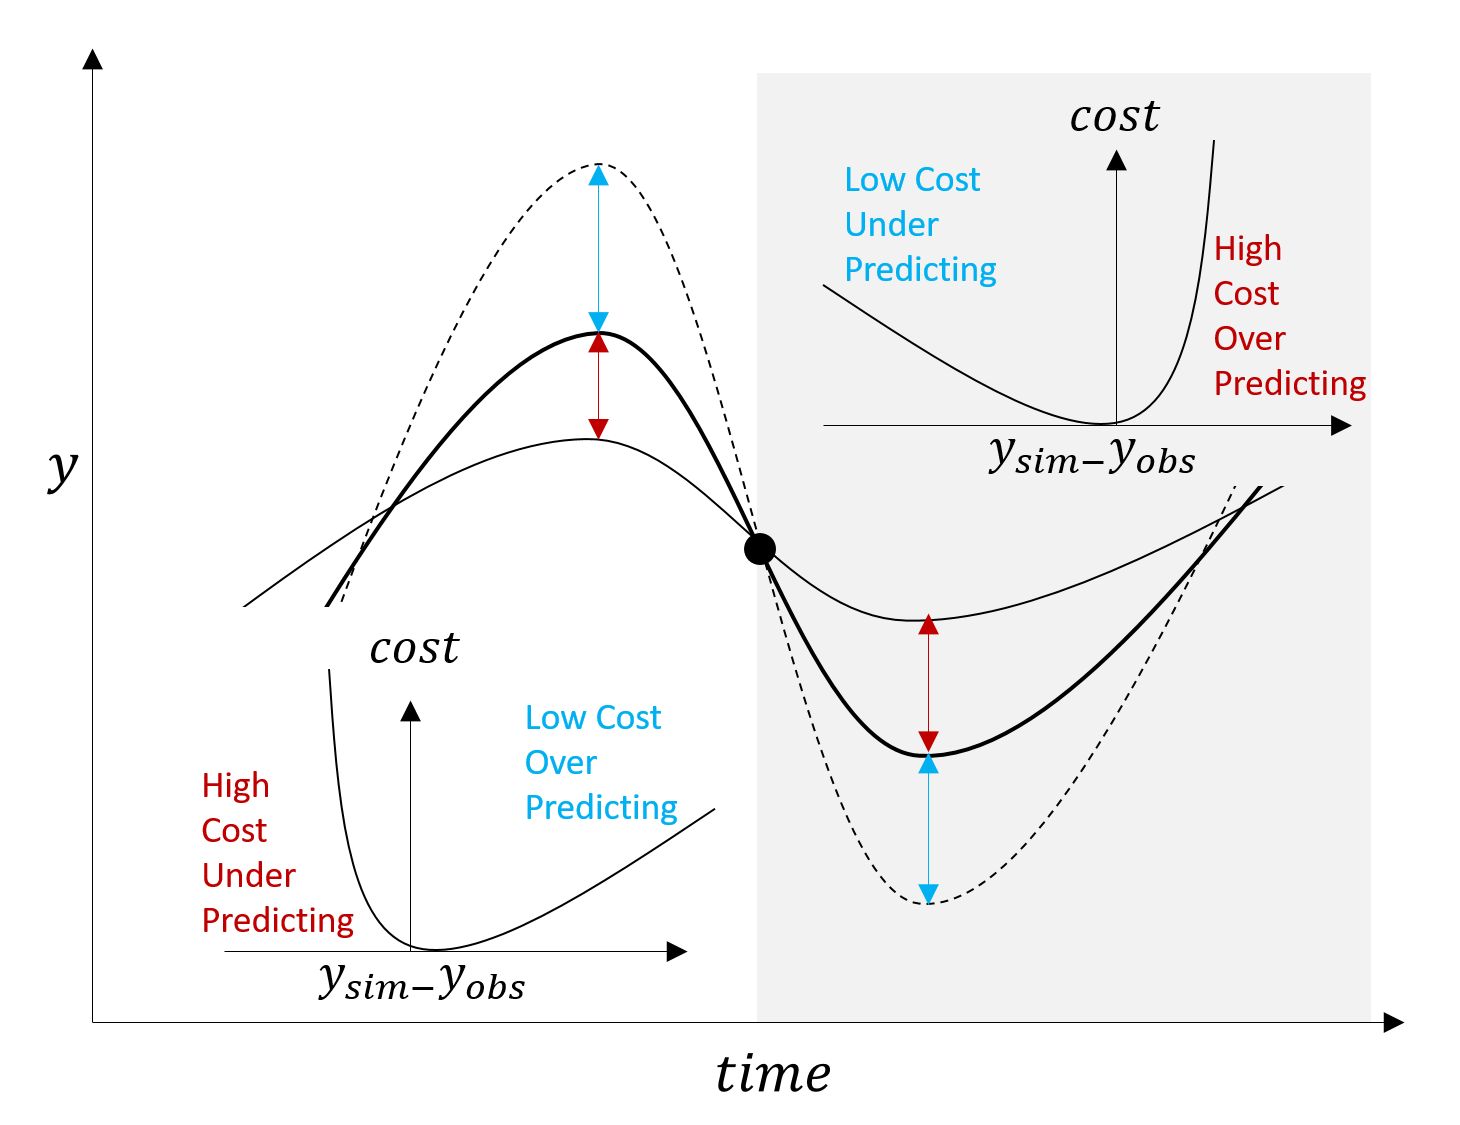
\includegraphics[width=\textwidth, trim={0 0 0 0}, clip=true]{plots/asymmetric1_b.png}
  		\caption{Asymmetric loss can be defined with LINEX functions.}
  		\label{fig:asymmetric1b}
	\end{subfigure}
	\caption{Asymmetric loss functions define different losses to over predicting and under predicting a value.}
	\label{fig:asymmetric1}
\end{figure}

\begin{equation} \label{eq:linex}
	LINEX(y_i,\hat{f}(x_i)) = e^{\phi(y_i-\hat{f}(x_i))} - \phi(y_i-\hat{f}(x_i))-1, \quad\text{$\phi$} \in \mathbb{R}
\end{equation}

\begin{figure}[ht]
	\centering
 	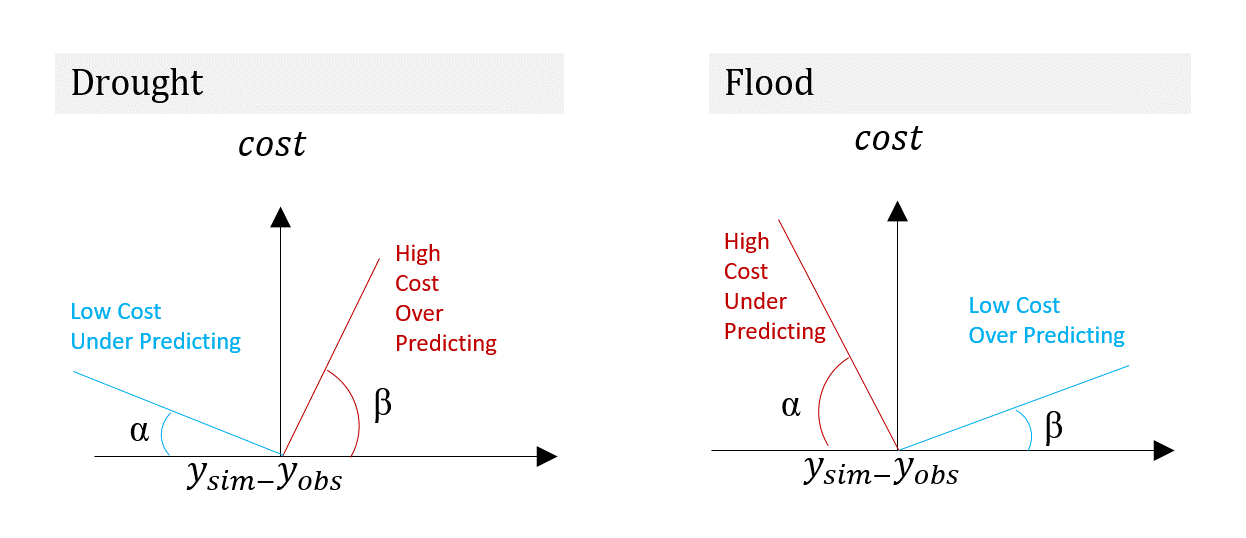
\includegraphics[width=0.8\textwidth, trim={0 0 0 0}, clip=true]{plots/asymmetric3.png}
	\caption{Asymmetric loss functions define different losses to over predicting and under predicting a value.}
	\label{fig:asymmetric3}
\end{figure}

\begin{equation} \label{eq:asshinge}
	Hinge(y_i,\hat{f}(x_i)) = \alpha*min(0, \hat{f}(x_i)-y_i)+ \beta*max(0, \hat{f}(x_i)-y_i)
\end{equation}

The squared error loss penalizes larger errors more than smaller error (i.e., the function is steeper in the tails than in the middle). To preserve this feature we can combine the concepts above and define a weighted $\ell2-norm$ (See Equation \ref{eq:weightedse}). 

\begin{equation} \label{eq:weightedse}
	Weighted\ Squared\ Error(y_i,\hat{f}(x_i)) = \alpha*\left[min\left(0, (\hat{f}(x_i)-y_i)\right)\right]^2+ \beta*\left[max\left(0, (\hat{f}(x_i)-y_i)\right)\right]^2
\end{equation}

%Also, we could develop a cost function that penalized a standard deviation ratio (See Equation \ref{eq:rsd}) greater than one more than it does the same measure when it is less than one (See Figure \ref{fig:asymmetric2}). Such a cost function will ensure we make more conservative decisions as over predicting extremes is valued over under predicting them.  
%
%\begin{figure}
%	\centering
%	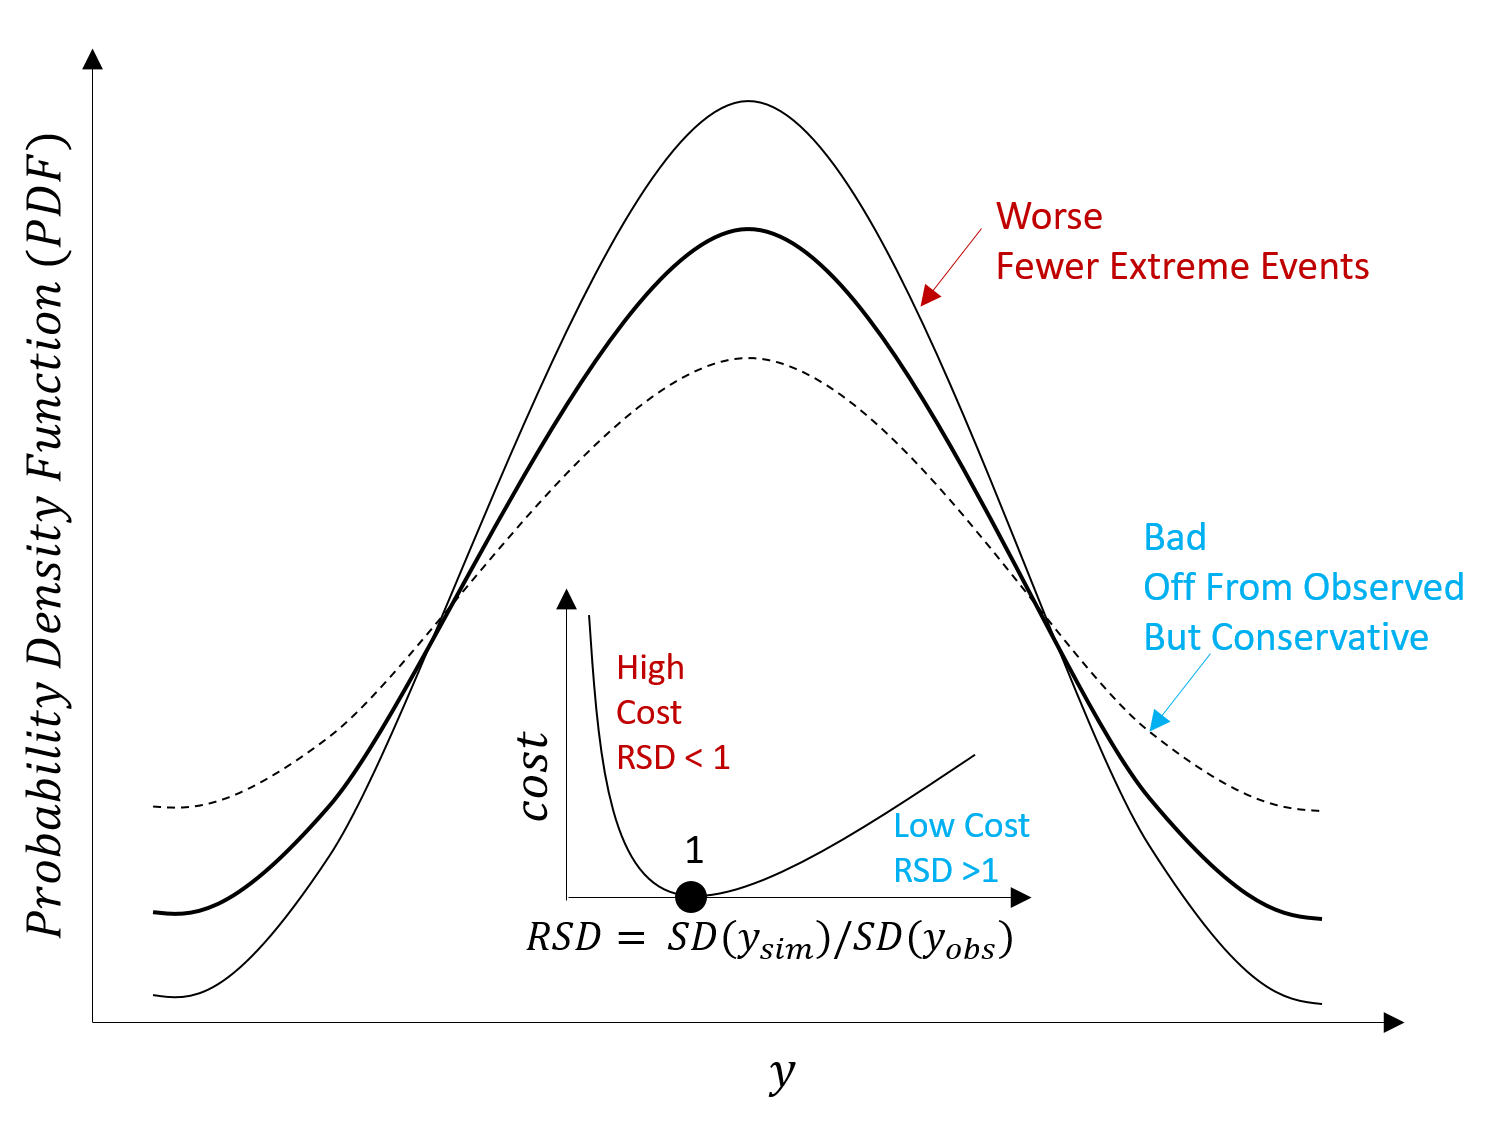
\includegraphics[width=.5\textwidth,trim={0 0 0 0},clip=true]{plots/asymmetric2.png}
%	\caption{ blah blah blah blah  blah blah blah blah  blah blah blah blah  blah blah blah blah  blah blah blah blah  blah blah blah blah} 
%	\label{fig:asymmetric2}
%\end{figure}

(2) \textbf{Should we be concerned with relative errors or absolute errors?} In hydrology, both manual and automatic attempts aimed at minimizing absolute errors often lead to fitting the higher portions of the hydrograph (i.e., peak flows) at the expense of the lower portions (i.e., baseflow) \cite{krause2005comparison}. Relative errors are generally more important than absolute errors. For example, a 10 TAF error in 1,800 TAF (monthly annual average of the Sacramento River) is less extreme of an error than in 15 TAF (monthly annual average of the Colorado River). Relative error loss functions or a simple log transformation of the data can help in this regard. 
% studentized, standardized by mean or sd? how are these different? 
% although for the matter for water supply then the absolute values are important not relative. 

(3) \textbf{Should losses be a continuous function, or stepwise?} Although, most outcomes may follow a discontinuous step function (e.g., a neuron firing or not), many decisions in water resources (e.g., releases from a reservoir) are continuous. Continuity and differentiability make continuous math more convenient. One major development in neural networks was doing away with the concept of thresholds in the step function (representing the collective influence of all the inputs) and replacing it with a smoother \textit{sigmoid} function. As with neural networks, many optimization algorithms require continuity and differentiability (e.g., gradient decent). However, advances in these methods now allow for piece-wise differentiability in the loss function.
% many different shapes in the loss function.

(4) \textbf{Should losses be homogeneous or heterogeneous (i.e., weighted based on geographic region)?} The cost of incorrectly managing a densely populated urban basin may be very different than a desert or a headwater basin; the importance of having accurate flow estimates is not completely homogeneous especially across a big and diverse region as California. However, to avoid making those judgements, we will use a single loss function across all regions. 
% could use cost functions that differentiate between the costs of predicting the wrong hydrology for a populated basin and the same costs for fish species. % should costs from CALVIN? cost of not delivering the target demand. is that the same cost as not predicting the hydrology right? not really. 

\citeA{legates1999evaluating} suggests that a complete assessment of model performance should include at least one \textit{goodness-of-fit} or relative error measure (e.g., Modified NSE or Modified d defined in Equation \ref{eq:mnse} \& \ref{eq:md}, with $j=1$) and at least one absolute error measure (e.g., RMSE or MAE defined in Equation \ref{eq:rmse} \& \ref{eq:mae}) with additional supporting information (e.g., a comparison between the observed and simulated mean and standard deviations such as those defined in Equation \ref{eq:rsd} \& \ref{eq:rmu}) \cite{legates1999evaluating}. 

Therefore, along with the four characteristics discussed above, we propose to use only the following three selected measures-of-fit: the Modified NSE (as a relative error measure), the MSE and weighted MSE (as an absolute error measure), and the RSD (as an additional supporting measure). 

%-----------------------------------------------------------------------------------------------------------------------------------------------------------------------------------------------------
%\section{Preliminary Results} \label{ch4:results}
%A main feature of L2 is its convexity, which means that the differences
%between high prediction errors are assessed as more important than differences
%between small prediction errors.
%even if there are strong arguments in a particular situation
%that the loss function should be convex, it is almost always impossible to find
%decisive arguments why it should be exactly equal to L2.

%-----------------------------------------------------------------------------------------------------------------------------------------------------------------------------------------------------
\section{Conclusion} \label{ch4: conclusion}
This chapter will follow a risk minimization framework in developing a loss function. Contrary to other studies, we \textit{are putting the horse before the cart}. That is, the loss function is developed before performing the learning, not just as an evaluation step after. The different performances of the models will be compared against the loss functions applied. Next, we will compare the shape of the predictions in the time-series compared to the observations. In squared error loss functions (i.e., MSE, NSE) the peaks get fitted at the expense of the low flows (i.e., high leverage points). However, the proposed wighted squared error asymmetric loss may be able to force a fit to both tails of the distribution. A comparison of the results from these losses will determine whether the aforementioned problem is mitigated with asymmetric losses. A dissertation chapter will include a comparison between the results of various loss functions applied. It will investigate the differences in the general shape of predictions obtained across the various loss functions, and discuss the effects of different weights in the asymmetric weighted MSE function.   

%Surprisingly, the models perform vastly different from one another depending on the objective function used, highlighting the importance of this much overlooked step. In summary, we define what loss means to a certain problem, we use that as the objective function in the machine learning algorithm, and then perform the minimization. 

% happy models are all alike, every unhappy model is unhappy in its own way.  

% add the table made for presentation here. Complete this table and the chapter will be finished. 

